A complete execution demo can be found at \href{https://usi365-my.sharepoint.com/:v:/g/personal/costafr_usi_ch/EVE8wwhO59xGo5FCfr8ZFvoBqFdS82ZzTcjgIl_GgPMrJQ?e=QbyhVj}{this link}.

\subsection{Successful outcomes}
The final implementation of the project is able to produce results matching our initial set of requirements in a satisfactory way. The robot in fact capable of, thorugh path planning, reach the position of all towers on the scene. Once the robot is in the vicinity of the tower it then proceeds to orbit around the perimeter of the target in search of the weak-spot (largest flat side). Finally the robot aligns itself to the face of the tower and the action of shooting a projectile towards it is simulated by creating a sphere with adequate mass and velocity.

\begin{figure}[H]
    \centering
    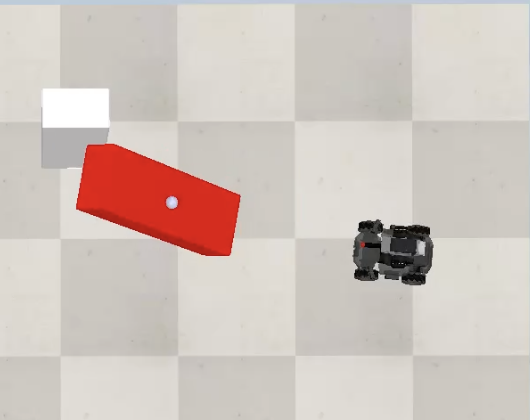
\includegraphics[width=0.3\textwidth]{Images/snapshot_shooting.png}
    \caption{Snapshot of the robot after shooting a projectile.}
    \label{fig:shooting}
\end{figure}

\subsection{Known Issues and Limitations}

While the system fulfils all the baseline requirements, in repeated trials we observed a handful of non‑deterministic failure modes that still require attention:

\begin{itemize}
    \item \textbf{Duplicate \texttt{/goal\_reached} notifications:} Under rare circumstances the topic remains latched and publishes the same message multiple times, leading either to redundant replanning or, conversely, to the node skipping the transition to the next goal.
    \item \textbf{Interleaved sensor callbacks during path execution:} While the robot is orbiting a tower, newly received range data can prompt the planner to generate a fresh trajectory that conflicts with the active controller, producing brief oscillations and jerky motion.
    \item \textbf{Odometry drift after collisions:} Odometry is calculated solely by double‑integrating wheel accelerations; an unexpected collision is therefore interpreted as free motion, causing the estimated pose to diverge from the true pose for the remainder of the run.
    \item \textbf{Weak‑spot detector sensitivity:} Strong glare or partial occlusion can distort the binarisation mask and cause the largest face to be mis‑identified, preventing proper alignment.
\end{itemize}